L'attenzione riservata all'elaborazione parallela da parte della comunit\'a
scientifica risale al 1957, anno in cui la
Compagnie des Machines Bull (l'odierna Bull SAS) ha annunciato Gamma 60, un computer \textit{mainframe}
equipaggiato con la prima architettura della storia in grado di offrire un supporto diretto
al parallelismo, mentre l'anno successivo, i ricercatori IBM John
Cocke e Daniel Slotnick hanno per la prima volta aperto alla
possibilit\'a di impiegare il \textit{parallel computing} per
l'esecuzione di simulazioni numeriche \cite{Wilson1994}.

\subsection{Alcune applicazioni del calcolo parallelo}
Oggi permangono applicazioni in ambito scientifico
che possono essere eseguite
solo su \textit{cluster} di elaboratori oppure che richiedono lo sviluppo di architetture specifiche di dominio (DSA, \textit{Domain Specific Architecture}), considerate le loro caratteristiche \textit{compute-intensive}.\newline
Esempi di settori che hanno beneficiato dello sviluppo di
architetture innovative per il calcolo parallelo sono la
bioinformatica, l'elaborazione di immagini e video
e il settore aerospaziale, che ha potuto contare su simulazioni
numeriche sempre pi\'u accurate.

La rivoluzione introdotta dal calcolo parallelo non si limita esclusivamente al campo scientifico: un dominio applicativo che negli ultimi due decenni ha registrato uno sviluppo senza precedenti \'e l'intelligenza artificiale (AI, \textit{Artificial Intelligence}) e, in particolare, l'addestramento di modelli di AI mediante tecniche di \textit{Machine Learning}. \newline
I successi e le evoluzioni ottenuti in questo settore, e tangibili in diversi campi di applicazione come il riconoscimento di oggetti o l'industria della traduzione, non sarebbero stati fattibili se non supportati da sistemi di calcolo sufficientemente potenti e in grado di eseguire le operazioni aritmetiche richieste dallo svolgimento di compiti sempre pi\'u complessi.

Come ulteriore esempio, possiamo citare i calcolatori dei moderni centri di calcolo, chiamati \textit{Warehouse Scale Computer} (WSC), che costituiscono l'infrastruttura di erogazione dei moderni servizi Internet utilizzati ogni giorno da milioni di utenti, come i motori di ricerca, i \textit{social network} e i servizi di \textit{e-commerce}.\newline
Inoltre, la rivoluzione del \textit{cloud computing}, ovvero l'offerta via Internet di risorse di elaborazione \enquote{\textit{as a service}}, consente l'accesso ai WSC a chiunque sia dotato di una carta di credito.
\subsection{La barriera dell'energia}
\nocite{Spirito2021}
Il fattore fondamentale dietro all'adozione di massa delle architetture multiprocessore \'e la riduzione del consumo di energia elettrica offerta dai sistemi di calcolo paralleli; infatti, l'alimentazione e il raffreddamento delle centinaia di server presenti in un centro di calcolo moderno costituiscono una componente di costo non trascurabile, che risente solo marginalmente della disponibilit\'a di sistemi di raffreddamento dei microprocessori adatti a dissipare una grande quantit\'a di energia.

Il consumo di energia elettrica dei microprocessori viene misurato in Joule (\si{J}) ed \'e quasi interamente rappresentato dalla dissipazione di energia dinamica da parte dei transistori CMOS (\textit{Complementary Metal Oxide Semiconductor}), essendo la tecnologia dominante impiegata nella realizzazione dei moderni circuiti integrati.
Un transistore assorbe prevalentemente energia elettrica durante la commutazione alto-basso-alto del suo stato di uscita, secondo la formula
$$
    E = V^{+2} \cdot C_{L}
$$
dove $E$ rappresenta l'energia dissipata nelle due transizioni, $V^{+}$ la tensione di alimentazione e $C_{L}$ la capacit\'a di carico del transistore.\newline
La potenza dissipata $P_{D}$, assumendo che la frequenza di commutazione dello stato del transistore sia pari a $f$, \'e quindi data da
$$
    P_{D} = f \cdot E = f \cdot C_{L} \cdot V^{+2} \propto f_{C}
$$
dove $f_{C}$ \'e la frequenza di \textit{clock} del circuito, esprimibile in funzione di $f$.

In passato, i progettisti di circuiti integrati hanno tentato di contenere l'assorbimento di energia da parte dei microprocessori riducendo la tensione di alimentazione $V^{+}$ di circa il $15\%$ ad ogni nuova generazione di CPU, fino al raggiungimento del limite inferiore di 1 $\si{V}$.\newline
Al contempo, la diminuzione della tensione di alimentazione ha favorito la crescita delle correnti di dispersioni interne al transistore, tanto che nel 2008 circa il $40\%$ della potenza assorbita da un transistore era imputabile alle correnti di dispersione; ci si \'e imbattuti in una vera e propria \enquote{barriera dell'energia}.

In figura \ref{fig:PrestazioniProcessori}, possiamo notare come fino alla prima met\'a degli anni Ottanta del secolo scorso, la crescita annua delle prestazioni dei processori si attestava al $25\%$, per poi passare al $52\%$ grazie a importanti innovazioni nella progettazione e nell'organizzazione dei calcolatori; infine dal 2002, si sta continuando a registrare una crescita delle prestazioni meno evidente, pari al $3.5\%$ annuo, a causa del raggiungimento dei limiti relativi la potenza assorbita.\newline
La presenza di queste limitazioni tecnologiche ha accelerato la ricerca di nuove architetture per microprocessori, culminata con lo sviluppo del primo processore \textit{multicore}, IBM Power4, nel 2001 e il successivo lancio delle prime CPU \textit{multicore} destinate al mercato \textit{consumer}, nel 2006 da parte di Intel e AMD.
\begin{figure}[htbp]
    \centering
    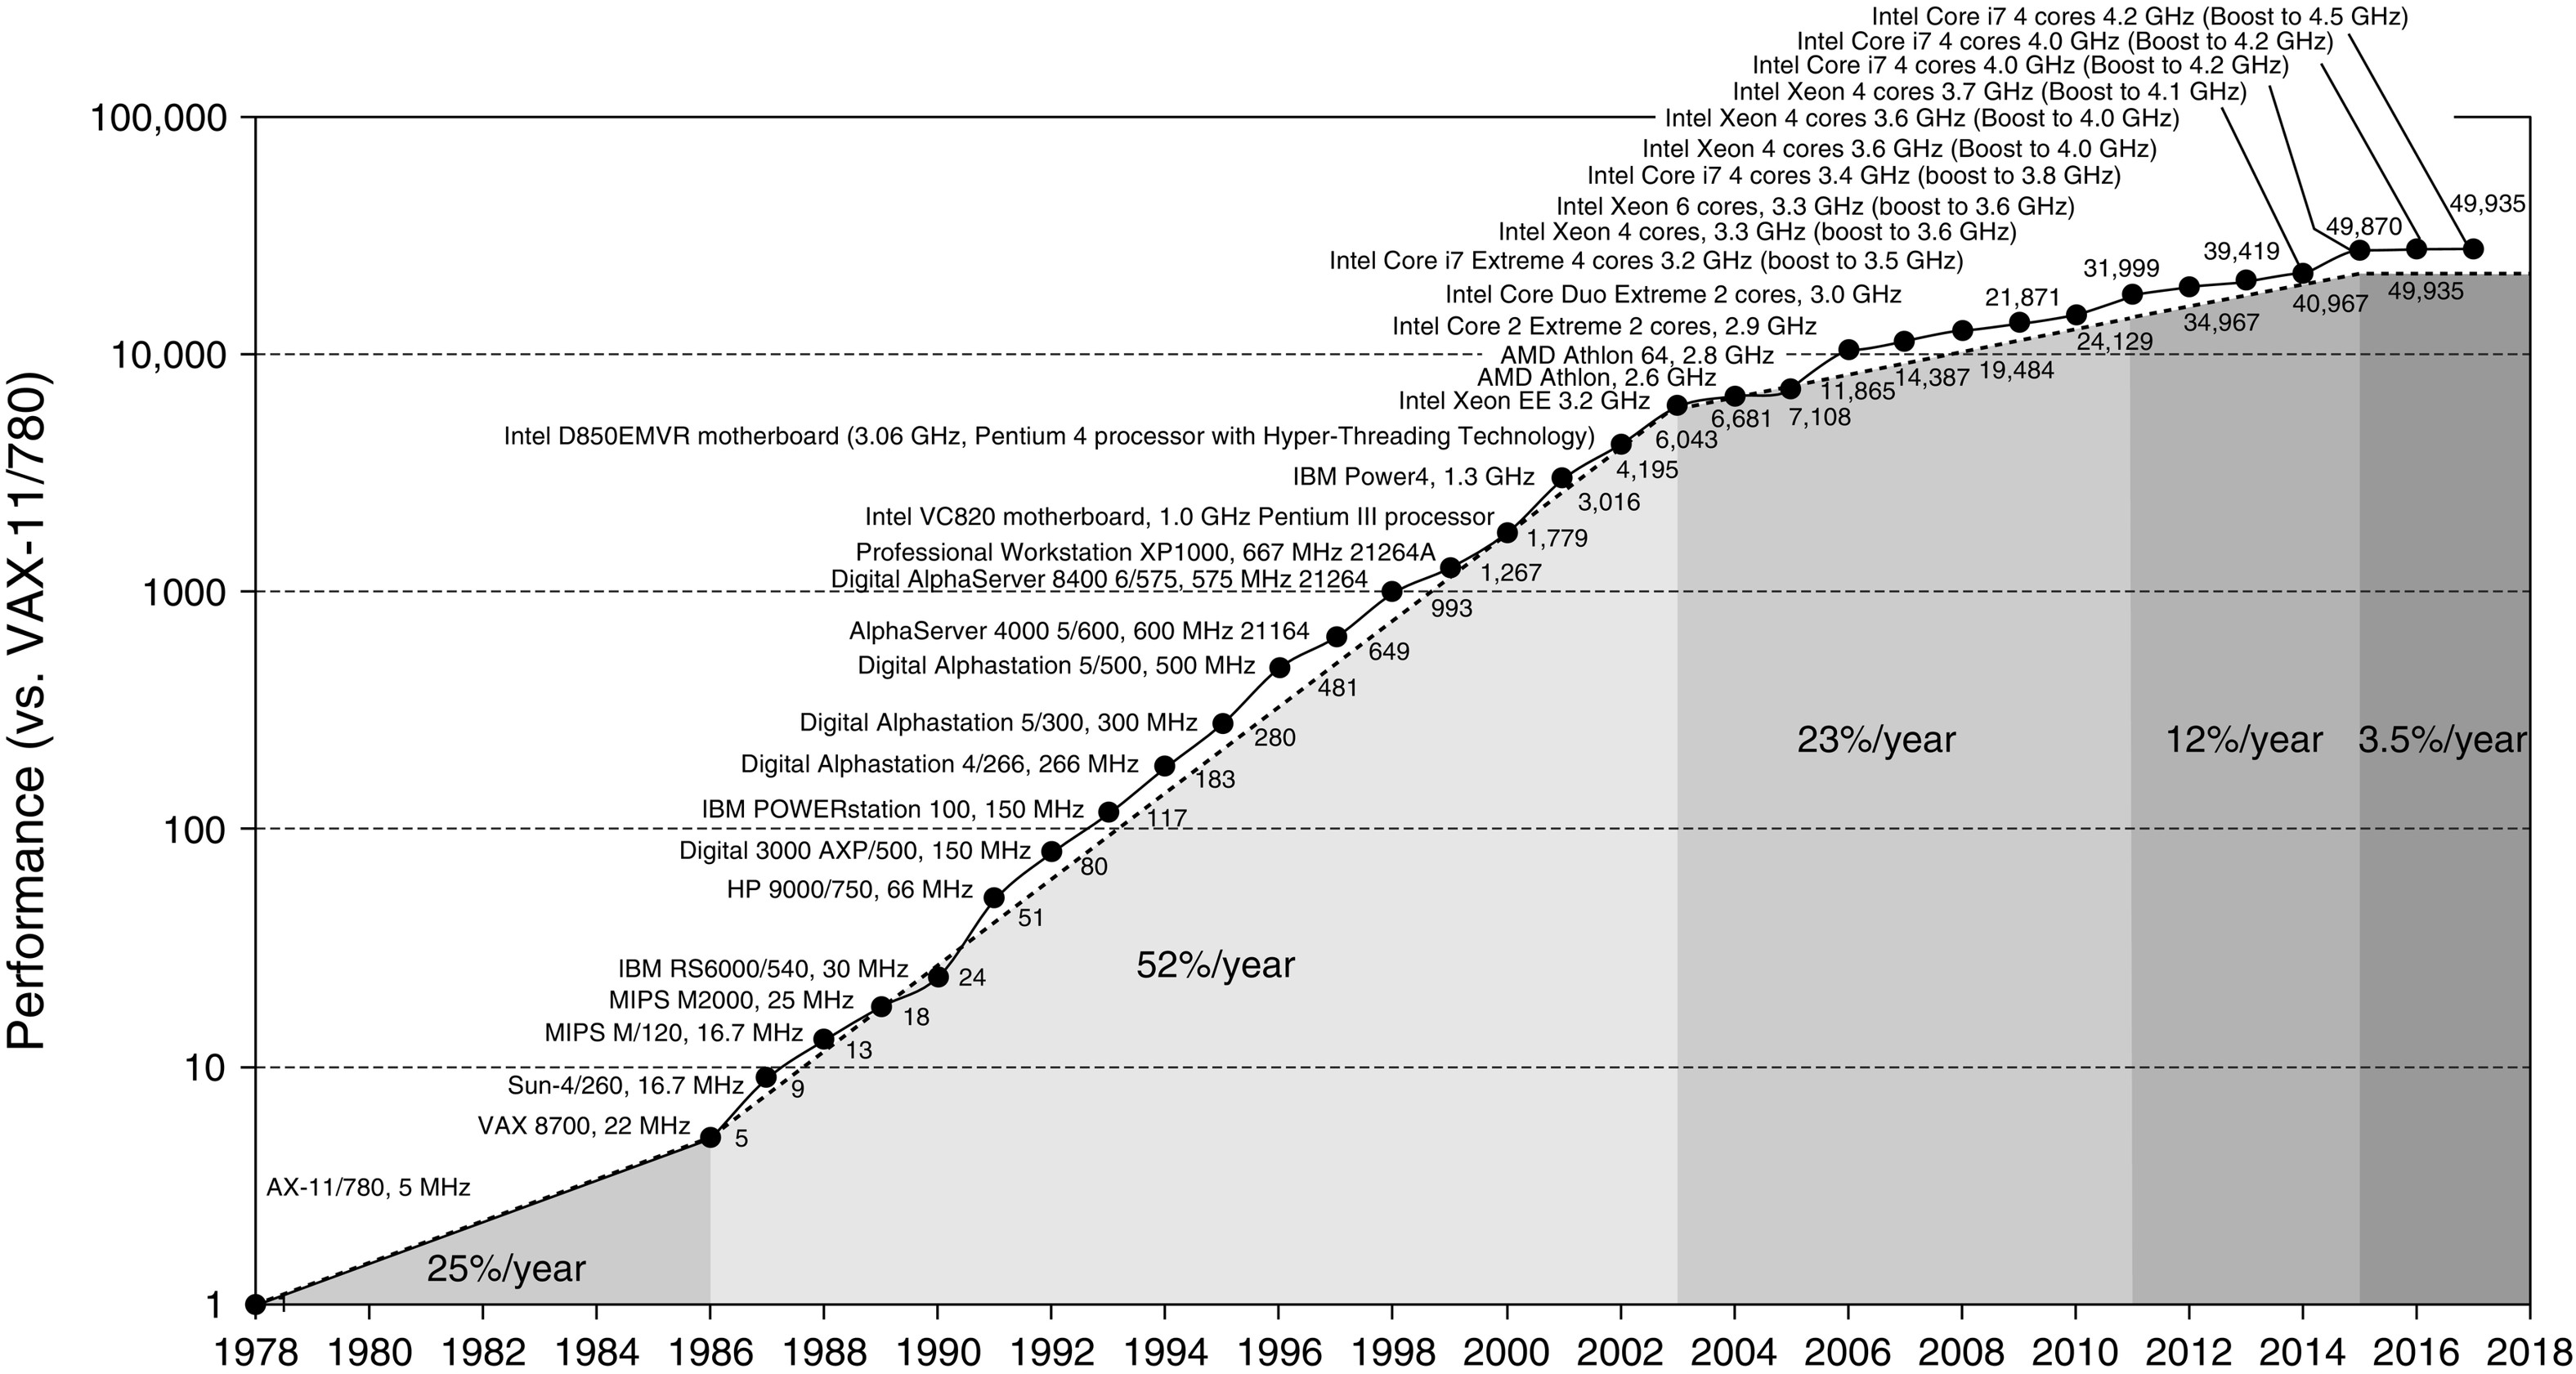
\includegraphics[width=0.8\textwidth]{../Immagini/Capitolo 1/PrestazioniProcessori}
    \caption{Crescita nelle prestazioni dei processori dal 1978 al 2018; il grafico riporta le prestazioni dei processori, paragonandoli al VAX11/780 mediante l'esecuzione dei \textit{benchmark} SPECint \small{\textit{(Da J.L. Hennessy, D.A. Patterson, Computer Architecture: A quantitative Approach. Ed. 6. Waltham, MA:Elsevier, 2017)}}}
    \label{fig:PrestazioniProcessori}
\end{figure}

In futuro, il miglioramento delle prestazioni dei microprocessori sar\'a verosimilmente apportato dall'aumento del numero di \textit{core} montati su un singolo \textit{chip} piuttosto che dalla crescita della frequenza di clock dei singoli processori.